% !TeX spellcheck = en_GB 
\documentclass[a4]{article}
%\usepackage[draft]{graphicx}

\usepackage{bold-extra}
\usepackage{ifthen}
\usepackage{graphicx}
\usepackage{epstopdf}
\usepackage{keylogo}
\usepackage{hyperref}
%\usepackage{a4}
\usepackage{listings}
\usepackage{amsmath}
\usepackage{amsfonts}
\usepackage{amssymb}
\usepackage{ifthen}
\usepackage{color}
\usepackage{subfigure}
\usepackage{booktabs}
\usepackage{microtype}
\usepackage{xspace}

\lstdefinelanguage{KeYJava}[]{Java}{%
  morekeywords={skip},
  otherkeywords={method-frame,Throwable,java.lang.Throwable,Object,Exception},
}

% attention! this is overriden elsewhere
\lstset{language=KeYJava, basicstyle=\ttfamily\upshape, 
  keywordstyle=\ttfamily\bfseries}


\setcounter{tocdepth}{2}
%   Christian Engel, Andreas Roth, Abian Blome, \\
%   Richard Bubel, Simon Greiner, Mattias Ulbrich, \\
%   Moritz von Looz, Sarah Grebing\\[0.5em]

\author{The \KeY{} Team\\
  \emph{This article is a variant of~\cite{umlkeyquicktour} by} \\
    \emph{Thomas~Baar, Reiner~H\"ahnle, and Steffen~Schlager.}  
}

\date{\today}

%\input{sga}

\title{\KeY\ Quicktour for JML \\ {\footnotesize Work in progress}}

\newcommand{\todo}[1]{{\large \bf TODO:{#1}}}

%\newcommand{\together}{Together\textregistered}
\newcommand{\together}{\textsc{TogetherCC}}
% Names of the  Together menus (diagrams, etc), also used for
% entries of the KeY-Prover
\newcommand{\tn}[1]{{\em #1}}

% Names of the product we are talking about
\newcommand{\kt}{\KeY\ tool}
\newcommand{\kp}{\KeY\ prover}
\newcommand{\javaWS}{Java Web Start}

\newcommand{\pob}{{\sf Proof Obligation Browser}}
\newcommand{\prm}{{\sf Proof Management}}
\newcommand{\ctCfg}{{\sf Contract Configurator}}

\newcommand{\self}{\mathit{self}}
% Name of the Java (UML) code
\newcommand{\jn}[1]{\texttt{#1}}

% How to emphasize spezifikation code
\newcommand{\spec}[1]{\texttt{#1}}

% entries of menus
\newcommand{\mea}[1]{\textsf{\textbf{#1}}}
\newcommand{\meb}[2]{\textsf{\textbf{#1}} $|$ \textsf{\textbf{#2}}}
\newcommand{\mec}[3]{\textsf{\textbf{#1}} $|$ \textsf{\textbf{#2}} $|$ \textsf{\textbf{#3}}}
\newcommand{\med}[4]{\textsf{\textbf{#1}} $|$ \textsf{\textbf{#2}} $|$ \textsf{\textbf{#3}} $|$ \textsf{\textbf{#4}}}

%%%%  Abkuerzungen zur Notation der Beweisverpflichtungen

\newcommand{\inv}{INV}
\newcommand{\pinv}[1]{INV^{P_{#1}}}

\newcommand{\pre}{m.PRE}
\newcommand{\ppre}[1]{m.PRE^{P_{#1}}}

\newcommand{\post}{m.POST}
\newcommand{\ppost}[1]{m.POST^{P_{#1}}}

\newcommand{\parent}[1]{P_{#1}}

\newcommand{\renameforpre}[1]{rename(#1)}

\newcommand{\allq}[2]{\forall {#1\ifthenelse{\equal{#2}{}}{}{\!\!:\!#2}}\,\,}
\newcommand{\dldia}[2]{\ensuremath{\langle#1\rangle{#2}}}  % DL formula dia
\newcommand{\dlbox}[2]{\ensuremath{[#1]{#2}}}  % DL formula box

\newcommand{\keyand}{\ensuremath{\mathrel{\&}}}
\newcommand{\keyor}{\ensuremath\mathrel{|}}
\newcommand{\keynot}{\ensuremath{\mathop{!}}}
\newcommand{\keyimplies}{\ensuremath{\mathrel{-\!\!\!>}}}
\newcommand{\keyequiv}{\ensuremath{\mathrel{<\!\!\!-\!\!\!>}}}
\newcommand{\keyif}{\ensuremath{\mathop{\text{if}}}}
\newcommand{\keythen}{\ensuremath{\mathop{\text{then}}}}
\newcommand{\keyelse}{\ensuremath{\mathop{\text{else}}}}
\newcommand{\keyeq}{\ensuremath{\doteq}}
\newcommand{\keyneq}{\ensuremath{\mathrel{{!}{\keyeq}}}}
\newcommand{\keyleq}{\ensuremath{\mathrel{<\!=}}}
\newcommand{\keygeq}{\ensuremath{\mathrel{>\!=}}}
\newcommand{\keygt}{\ensuremath{>}}
\newcommand{\keylt}{\ensuremath{<}}
\newcommand{\keyquantification}[3]{#1 
  {~#2 \ifthenelse{\equal{#3}{}}{}{~#3};~}}
\newcommand{\keyallq}[2]{\ensuremath{\keyquantification{\backslash\text{forall}}{#1}{#2}}}
\newcommand{\keyexq}[2]{\ensuremath{\keyquantification{\backslash\text{exists}}{#1}{#2}}}
\newcommand{\keyquantificationmath}[3]{#1 
  {\ifthenelse{\equal{#3}{}}{#2}{#3 : #2}.\,}}
\newcommand{\keyallqmath}[2]{\ensuremath{\keyquantificationmath{\forall}{#1}{#2}}}
\newcommand{\keyexqmath}[2]{\ensuremath{\keyquantificationmath{\exists}{#1}{#2}}}
\newcommand{\keytrue}{\mathop{\mathrm{true}}}
\newcommand{\keyfalse}{\mathop{\mathrm{false}}}

\newcommand{\elUp}[2]{\ensuremath{#1 := #2}}
\newcommand{\seqUp}[2]{\ensuremath{#1 \,; #2}}
\newcommand{\parUp}[2]{\ensuremath{#1 \,||\, #2}}
\newcommand{\quanUp}[3]{\ensuremath{\mathtt{for~}#1 ;\, #2 ;\, #3}}
\newcommand{\ifUp}[2]{\ensuremath{\mathtt{if~~}#1;\, #2}}
\newcommand{\applyUp}[2]{\ensuremath{\{#1\}\;#2}}




\hyphenation{paycard-Interactive}
\hyphenation{Java-CardDL}

\begin{document}

\maketitle

\section{Introduction}
\label{sec:introduction}

When we started writing this document, we aimed at providing a short
tutorial accompanying the reader at their first steps with the \KeY\
system. The \kt\ is designed as an integrated environment for
creating, analyzing, and verifying software models and their
implementation. The reader shall learn how to install and use the
basic functionality of the \kt. Besides practical advises how to
install and get \KeY\ started, we show along a small project how to
use the \kt\ to verify programs.

Verification means proving that a program complies with its specification
in a mathematically rigorous way. In order to fulfill this task, the
specification needs to be given in a formal language with a precisely
defined meaning. In the current version of the document, we focus on
the popular \emph{Java Modeling Language}
(JML)~\cite{JMLReferenceManual11,Leavens-Baker-Ruby04} as specification
language.

In the next sections, we show how to verify a JML-annotated (specified)
Java\-Card program. For this purpose, \KeY\ features a calculus for the complete
Java\-Card language including advanced features like transactions.

Besides JML, the \kt\ supports Java\-Card\-DL as a specification
language. 

For a longer discussion on the architecture, design philosophy, and
theoretical underpinnings of the \kt\, please refer to
\cite{KeYBook2016}.
%
In case of questions or comments, don't hesitate to contact the
\KeY support team at 
\href{mailto:support@key-project.org}{\emph{support@key-project.org}}.

\subsection{Version Information}
\label{sec:version}

This tutorial was tested for \KeY\ version 2.10.

\subsection{Installation}
\label{sec:install}

You can choose between different methods to install and use \KeY.
For this tutorial, we
recommend the \javaWS\ variant described in
Sect.~\ref{install:javaws}. 

\subsubsection{The \kp{} by \javaWS}
\label{install:javaws}

\javaWS\ is a Java Technology which allows you to start applications
directly from a website. No installation is needed. You can visit our
homepage
\begin{center}
  \url{http://www.key-project.org/download}
\end{center}
which contains a link to \javaWS\ the \kp.
%
Please note that you need the \javaWS\ facility
(which should come along with your Java distribution).

\subsubsection{Byte Code and Source Code Installation}
\label{install:byteandsourcecode}

The download site offers also the binary and source-code versions of
\KeY.

%\emph{Please note:} Support for Borland Together has been discontinued
%with \KeY~1.4.
% Nevertheless the code is still present and the basic
% functionality should work with the stand-alone (non-eclipse) versions
% of Together Solo or TogetherCC, but that is without guarantee. The
% bytecode resp.\ sourcecode version is required for the Borland
% Together plug-in.
        
% NOTE: The Eclipse plugin cant be used with latest Eclipse
%
% \subsubsection{The \KeY-plugin for Eclipse}
% \label{install:eclipse}
% 
% In this section we will describe how to setup the \KeY-plugin
% for Eclipse as well as the use of some of its core features.
% We assume that Eclipse has already been installed on the
% target computer. Start it and in the menu \emph{Help} select
% \emph{Software Updates} and then \emph{Find and Install}.
% In the new window activate \emph{Search for new features to
% install} and click on \emph{Next}. Now add the \emph{New Remote
% Site} \url{http://www.key-project.org/KeYDists/KeY_Feature/}
% with a name of your choice. 
% Click on \emph{Finish}. Now a new window should appear with
% a list of installable features. Mark \KeY\ and continue.
% After accepting the license agreement and selecting a usable location
% you will be asked to verify the installation. Do so by clicking on
% \emph{Install all} and restart Eclipse when asked to. This completes
% the installation. It is possible to update the \KeY-plugin by selecting
% \emph{Search for updates of the currently installed features} in the 
% \emph{Software updates} menu.
% You can now start the standalone version of the prover by either clicking
% on the \KeY\ logo in the menu bar or from the \emph{Verification} menu.


%%% Local Variables: 
%%% mode: latex
%%% TeX-master: "quicktour"
%%% End: 


\section{Tutorial Example}

\subsection{Scenario}
The tutorial example is a small paycard application consisting of two
packages \jn{paycard} and \jn{gui}. The \jn{paycard} package contains all
classes implementing the program logic and has no dependencies to the
\jn{gui} package.

\texttt{paycard} consists of the classes: \jn{PayCard},
\jn{LogFile}, and \jn{LogRecord}. \jn{gui} package contains \jn{ChargeUI},
\jn{Issue\-CardUI}, and the main class \jn{Start}. 

In order to compile the project, change to the \texttt{quicktour-2.0} directory and
execute the following command:

\verb+javac -sourcepath . gui/*.java+

\noindent Executing

\verb+java -classpath . gui.Start+

\noindent starts the application. Try this now\footnote{Potential
  warnings can be safely ignored here.}.

The first dialog when executing the main method in \jn{Start} asks the
customer (i.e., the user of the application) to obtain a paycard. A
paycard can be charged by the customer with a certain amount of money
and thereafter used for cashless payment until the pre-loaded money is
eaten up. 

To prevent any risk to the customer when losing the paycard, there
is a limit up to which money can be loaded or charged on the
paycard. There are three paycard variants
with different limits: a standard paycard with a limit of 1000, a junior
paycard with a limit of 100, or a paycard with a user-defined limit.
The initial balance of a newly issued paycard is zero. 

In the second dialog coming up after obtaining a paycard, the customer
may charge their paycard with a certain amount of money. But the charge
operation is only successful if the current balance of the paycard
plus the amount to charge is less than the limit of the
paycard. Otherwise, i.e., if the current balance plus the amount to
charge is greater or equal the limit of the paycard, the charge
operation does not change the balance on the paycard and an attribute 
counting unsuccessful operations is increased. 

The \kt\ aims to {\em formally prove} that the implementation actually
satisfies such requirements.  For example, one can formally verify the
invariant that the balance on the paycard is always less than the
limit of the paycard.

The intended semantics of some classes is specified with the help of
invariants denoted in the Java Modeling Language
(JML)~\cite{JMLReferenceManual11,Leavens-Baker-Ruby04}. Likewise, the
behavior of most methods is described in form of pre- and postconditions
in JML. We do not go into details on \emph{how} JML specifications
for Java classes are created. The tools downloadable from
\texttt{http://jmlspecs.org/download.shtml} may be helpful here. In
particular, \textbf{we require and assume that all JML specifications
  are complying to the JML standards}~\cite{JMLReferenceManual11}. \KeY's
JML front-end is no substitute for the JML parser / type checker.

% Together support discontinued
%
%The UML/OCL version of the \kt\ provides more support for creating a
%formal specification such as stamping out formal specifications from
%design patterns or natural language support~\cite{umlkeyquicktour}.

\subsection{A First Look on the JML Specification}
\label{tutorialExample:firstLook}

Before we can verify that the program satisfies the property mentioned
in the previous section, we need to express it in JML. The remaining
section tries to give a short, intuitive impression on what such a
specification looks like. In Sect.~\ref{sec:analyze}, JML
specifications are explained in a bit more depth.

Load the file \jn{paycard/PayCard.java} in an editor of your choice and search
for the method \jn{isValid}. You should see something like

\lstset{
  language=Java,
  columns=flexible,
  commentstyle=\ttfamily,
  keywordstyle=\ttfamily\bfseries
%  keywordstyle=\sffamily\bfseries
}

\begin{lstlisting}
        /*@
          @ public normal_behavior
          @ requires true;
          @ ensures \result == (unsuccessfulOperations<=3); 
          @ assignable \nothing;
          @*/
        public /*@pure@*/ boolean isValid() {
           if (unsuccessfulOperations<=3) {
              return true;
           } else {
              return false;
           }
        } 
\end{lstlisting}

JML specifications are annotated as special marked
comments in Java files. Comments containing JML
annotations have an ``at'' sign directly after the comment sign as a start
marker and---for multi-line comments---also as an end marker.

The JML annotation in the above listing represents a JML method
contract. A contract states that when the caller of a method ensures
that certain conditions (precondition + certain invariants (see
Sect.~\ref{sec:provableProp})) then the method ensures that after the
execution the postcondition holds\footnote{The complete semantics is
  more complex; see Sect.~\ref{sec:provableProp}
  and~\cite{JMLReferenceManual11}.}.

The precondition is \jn{true}. This means the precondition does not
place additional conditions the caller has to fulfill in order to be
guaranteed that after the execution of the method its postcondition
holds, though there might be conditions stemming from invariants.

The \jn{ensures} clause specifies the method's postcondition and
states simply that the return value of the method is \jn{true} if and
only if there have not been more than 3 unsuccessful
operations. Otherwise, \jn{false} is returned.

For the other parts of the method specification, see
Sect.~\ref{sec:provableProp}.


%%% Local Variables: 
%%% mode: latex
%%% TeX-master: "quicktour"
%%% End: 


%include{verificationGeneral}

\section{How to Verify JML Specifications with the \kt}
\label{sec:analyze}

JML specifications, in particular pre-~and postconditions, can be seen
as abstractions of an implementation.  In this context, an
implementation is called {\em correct} if it actually implies the
properties expressed in its specification. The \kt\ includes
functionality to {\em verify} the correctness of an implementation
with respect to its specification. 

In this section, we describe how to start (Sect.~\ref{sec:starting})
the \kp\ and load the tutorial example (Sect.~\ref{sec:loading}) as
well as a short overview about the graphical user interface and its
options (Sect.~\ref{sec:prover}). Last but not least, we explain
how to configure the \kp\ to follow the tutorial example
(Sect.~\ref{sec:configure}).


\subsection{Starting the \kp}
\label{sec:starting}

In order to verify a program, you first need to start the \KeY\
prover. This is done either by using the webstart mechanism (see
Sect.~\ref{install:javaws}) or by running the jar file from 
your \KeY\ distribution\footnote{In
  this case we assume that you have installed the \kt\ as described in
Sect.~\ref{install:byteandsourcecode}.}, e.g.,~by
running
  \begin{center}
    \texttt{java -jar key.jar} 
  \end{center}

% Eclipse is atm unsupported
%\noindent If you use the Eclipse intall, start the \kp\ as stand-alone tool via
%the menu \mea{Verification}. 

\subsection{Loading the Tutorial Example}
\label{sec:loading}

After downloading and unpacking this quicktour, you should find a
directory containing the two subdirectories
\texttt{paycard} and \texttt{gui}. We refer to the directory
\texttt{jml} as top-level directory.


\begin{enumerate}
\item You have to choose the Java source files you want to
  verify. They contain both the source code and the JML
  annotations. You can do this by either
\begin{itemize}
  \item adding the path to the \texttt{paycard}
    directory to the command:
    \begin{center}
      \texttt{java -jar key.jar <path\char`\_to\char`\_quicktour>/jml/paycard}  
    \end{center}
  \item opening \meb{File}{Load} and selecting the \texttt{paycard}
    package directory after having started \KeY\ without
    any arguments.
\end{itemize}

\KeY\ will then load the tutorial example and parse the JML
annotations. If you get an error dialog similar to the one in
  Fig.~\ref{fig:error:unknownType}, you have selected the
  \texttt{jml} directory instead of its subdirectory \texttt{paycard}.

\begin{figure}
\centering
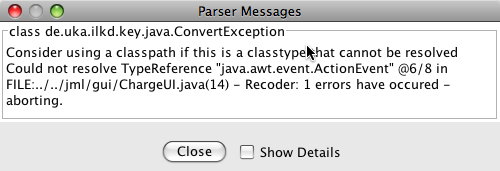
\includegraphics[width=0.75\textwidth]{../figures/errorDialogUnknownType}
\caption{Error dialog complaining about an unknown type}
\label{fig:error:unknownType}
\end{figure}

If you have your own projects you want to verify, you can proceed
similarly. Please note that \KeY\ by default supports only a very
limited selection of the standard library classes.
How to extend them and how to
configure more complex projects that use 3rd party libraries is
described in brief in App.~\ref{app:configuringProjects}.

\item Now the \prm{} window should appear as shown in
  Fig.~\ref{fig:pob:startup}.
  
  \begin{figure}[hp]
    \centering
    \subfigure[\pob\ after startup with expanded \jn{paycard}
    package\label{fig:pob:startup}]{ \centering
      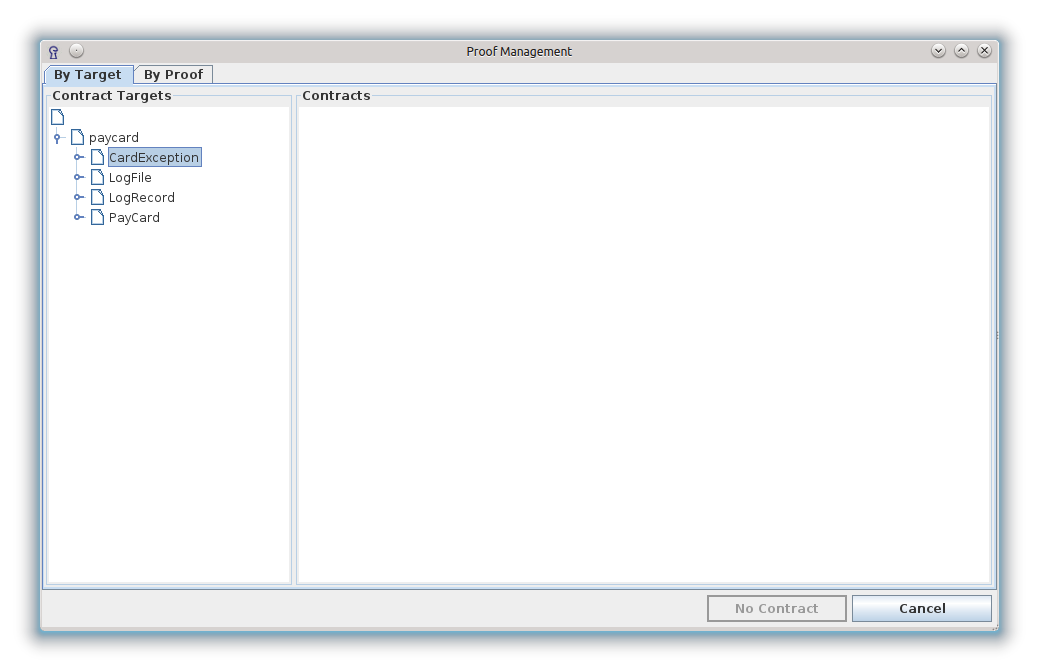
\includegraphics[width=\textwidth]{../figures/proofmanagement}
    }
    \subfigure[\pob\ listing proof obligations for \jn{PayCard::charge} \label{fig:pob:expandedProofObligations}]{
      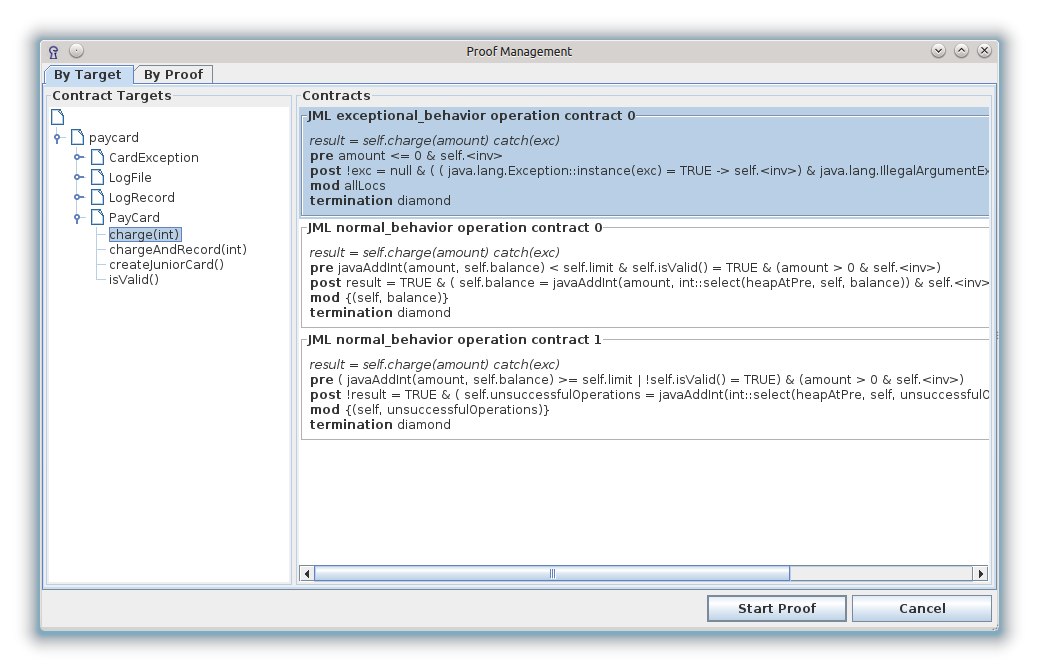
\includegraphics[width=\textwidth]{../figures/proofmanagement_paycard}
    }
    \caption{The \pob\ window}
    \label{fig:proofObligationBrowser}
  \end{figure}

  In the left part of the window titled \mea{Contract Targets},
  the \prm{} lists all packages, classes, interfaces, and methods of the
  project to be verified in a tree structure similar to standard file
  managers.

  The browser allows you to select the proof obligation you want to verify. 
  Selecting \jn{PayCard::charge} gives you three contracts
  (Fig.~\ref{fig:pob:expandedProofObligations}):
  one \mea{exceptional\_behavior}
  and two \mea{normal\_behavior} contracts. Select the first \mea{normal\_behavior}
  contract
  and confirm by pressing the button \mea{OK}. More details about the
  contract configurator will be given in Sect.~\ref{sec:provableProp}.

\item You should now see the \kp\ window with the loaded proof
  obligation as in Fig.~\ref{fig:proverWithLoadedPO}. The prover is
  able to handle predicate logic as well as dynamic logic. The \kp\
  was developed as a part of the \KeY project and is implemented in
  \textsc{Java}. It features interactive application of proof rules
  as well as automatic application controlled by strategies. In the
  near future more powerful strategies will be available.

  In Sect.~\ref{sec:application}, we show how to prove some of the
  proof obligations generated for the tutorial example.
\end{enumerate}

  \begin{figure}
    \centering
    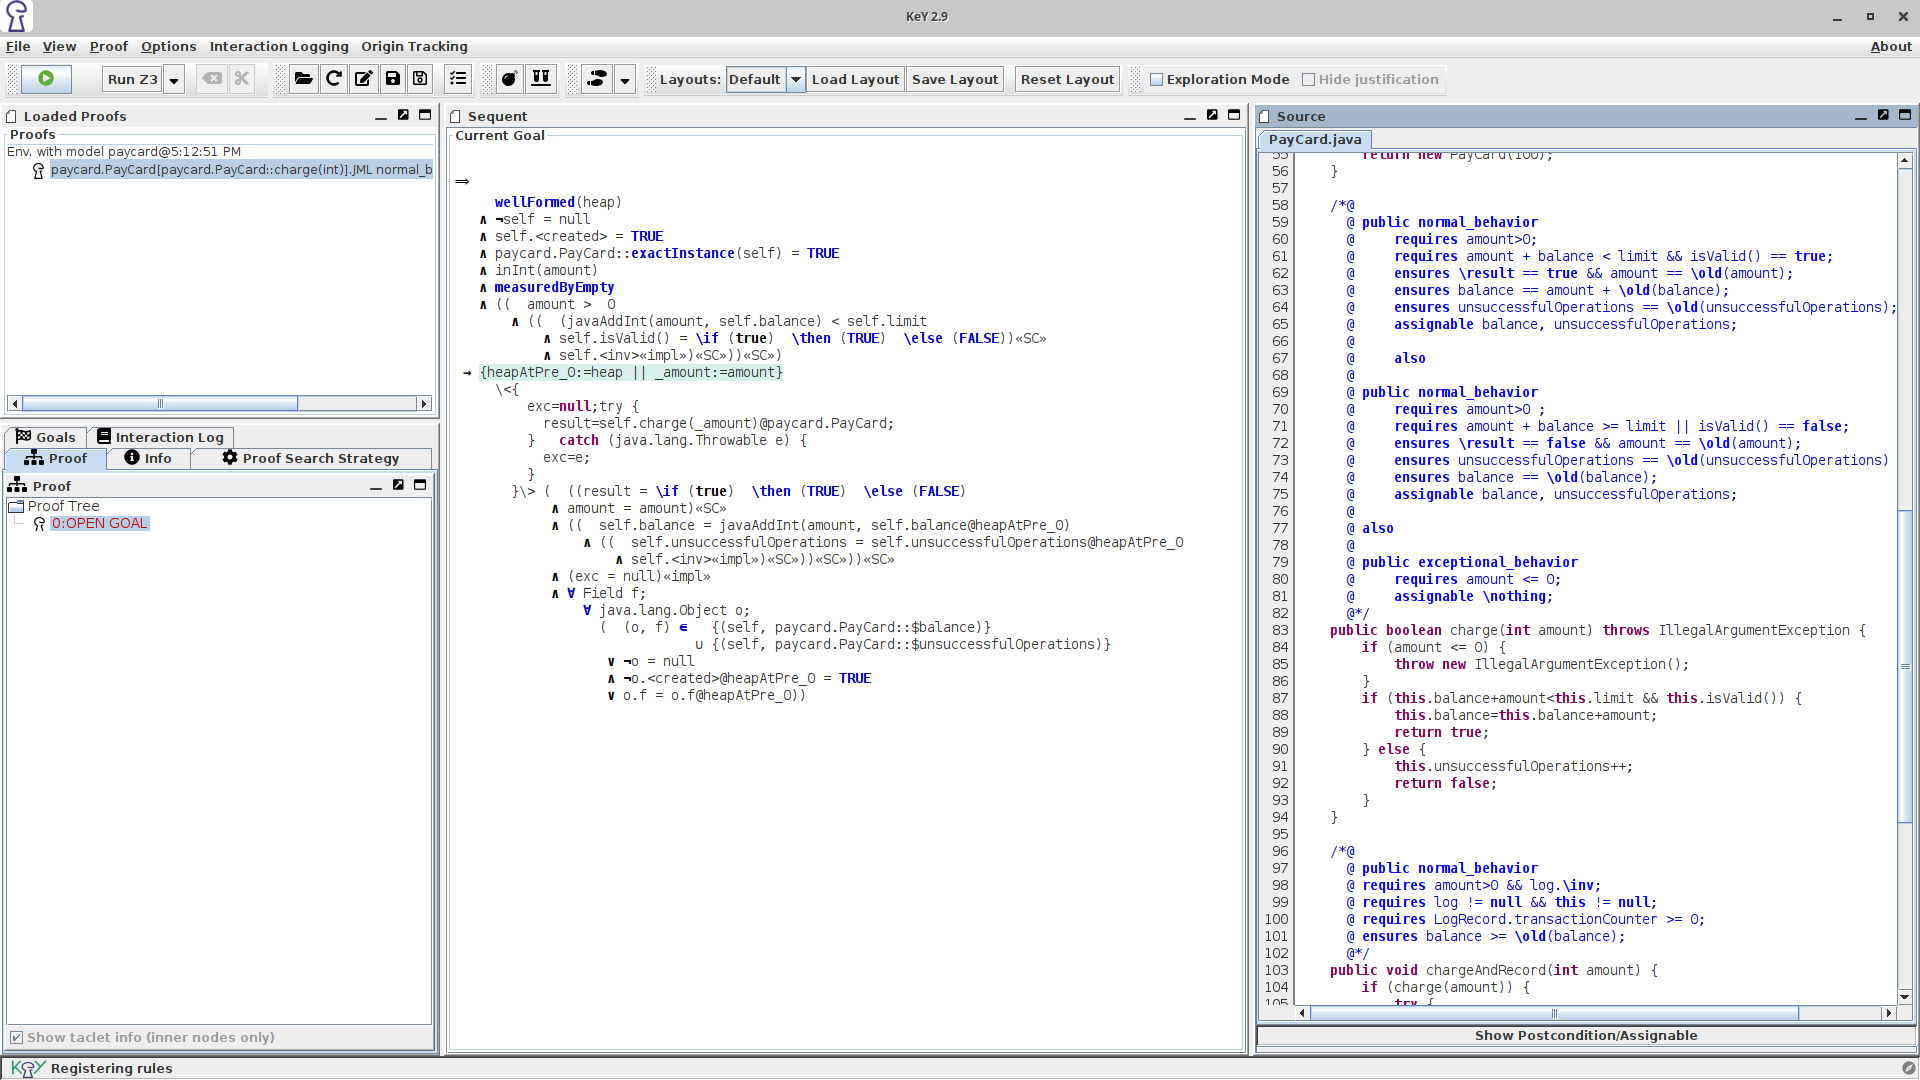
\includegraphics[width=\textwidth]{../figures/proverWithLoadedPO}
    \caption{The \kp\ with the contract
      for \jn{charge} loaded.}
    \label{fig:proverWithLoadedPO}
  \end{figure}


\subsection{The \kp} 
\label{sec:prover}

We assume that you have performed the steps described in the previous
section and that you see now something similar to
Fig.~\ref{fig:proverWithLoadedPO}. In this section, we describe the GUI
of the \kt\ and its different components. Most of the components in
the GUI are also labeled with a tooltip.


The \kp\ window consists of a menubar, a toolbar (all buttons explained in~\ref{app:shortcuts}) 
and three panes where 
the lower left pane is additionally tabbed. Each pane is described below.
%
The layout of the three panes can be changed by the user. Layouts can be saved and loaded
in the \meb{View}{Layout} menu.

\begin{description}

\item[Upper left pane:] Every problem you want to prove with the \kp\
is loaded in a proof environment. In this pane, all currently loaded
problems respectively their proof environments are
listed.


\item[Lower left pane:] This pane contains the following five tabs.
  
  \begin{description}
  \item[Proof:] This pane (see Fig.~\ref{fig:prover:tab:proof})
      contains the whole proof tree which represents the current
      proof. The nodes of the tree correspond to sequents (goals) at
      different proof stages. Click on a node to see the corresponding
      sequent and the rule that was applied on it in the following
      proof step (except if the node is a leaf). Leaf nodes of an open
      proof branch are colored red whereas leaves of closed branches
      are colored green.
    
      Pressing the right mouse button on a node of the proof tree will
      open a pop-up context menu. If you choose \tn{Prune Proof},
      the proof tree will be cut off at this node and all nodes lying
      below will be deleted. Choosing \tn{Apply Strategy} will start
      an automatic proof search (see later \tn{Automatic Proving}),
      but only on the branch which the node you had clicked on belongs to.
      
      The context menu also contains commands that allow you to hide
      closed subtrees, to hide inner nodes, to collapse, or to expand
      the tree. The commands help you to keep track of a large proof.
    
  \item[Goals:] In this pane, the open goals of a certain proof
    (corresponding to one entry in the upper left pane) are listed. To
    work on a certain goal just click on it and the selected sequent
    will be shown in the right pane.
    
%   \item[User Constraint:] To explain this functionality would go
%     beyond the scope of this quicktour. It won't be required in the
%     sequel.

  \item[Info:] In this pane (Fig.~\ref{fig:prover:tab:rules}), all the
    rules, term labels, and function symbols
    available in the system are indicated.
    
    For the rules, \KeY\ distinguishes
    between \tn{axiomatic taclets} (rules that are always true in the
    given logic), \tn{lemmas} (that are derived from and thus provable
    by axiomatic taclets) and \tn{built-in rules} (for example how
    certain expressions can be simplified).
    
    By clicking on a rule of the list, the description of that rule is
    shown in the box below the rule list.
    
    Term labels are additional information that can be attached to a term.
    They do not change a term's semantics, but are used to guide the poof
    search or to carry non-logical information about a term, like its
    corresponding line number in the source code.
    
    The function symbols folder lists all interpreted function and predicate
    symbols in the dynamic logic.
    
  \item[Proof Search Strategy:] This tab (see
    Fig.~\ref{fig:prover:tab:strategy}) allows you to define the active
    strategy from a set of available strategies. There are several
    parameters and only the most important ones will be covered here, 
    a complete list can be found in~\ref{app:strategy}:

    \begin{description}
%     \item[Autoresume strategy] By checking this you tell KeY to continue automated proof search after user interaction.

    \item[Max. Rule Applications] You can set the number $N_{aut}$ of
      automatic rule applications using the slider. Even if the
      automatic strategy can still apply rules after $N_{aut}$
      applications, automatic proving stops. 


    \item[Stop At] Choose when strategy execution shall stop.
      Possible values are \texttt{Default}: strategy stops when no
      rules are applicable or the maximal number of steps is reached and
      \texttt{Unclosable}: strategy stops in all situations when
      \texttt{Default} stops but also already when the first goal is
      encountered on which no further rule is (automatically) applicable. 

    \item[Proof splitting] Influences usage of rules branching a
      proof tree. Only rules working on formulas not on
      programs fall under the chosen policy, i.e., program rules
      causing
      splits are still applied even if splitting is switched off. The
      values are \texttt{free} (withour restrictions), \texttt{Delayed}
      (allows still splitting but prefers other rules) and \texttt{Off} (no
      splitting).

    \item[Loop treatment] This setting determines how while-loops are
      treated. They can be left untouched (\texttt{None}), handled
      using stated invariant contracts, or
      repeatedly unrolled (\texttt{Expand}). If handled using invariants,
      you can either choose the new \texttt{Loop Scope} rule (recommended),
      or the legacy \texttt{Transformation}-based rule.

    
    \item[Method treatment] Methods can also be left untouched
      (\texttt{None}), have their method contracts applied
      (\texttt{Contracts}), or be inlined, i.e. have the method body
      expanded in place (\texttt{Expand}).
      
    \item[Dependency contract] For the simplification of heap terms, setting this option to \texttt{On}
				the information in JML's \texttt{accessible} clause is used. 

   \item[Arithmetic treatment] The \kp\ has several options for the treatment of arithmetic expressions:
   \begin{description}
   \item[Basic:] Using this option, polynomial expressions are simplified. 
		 In the antecedent Gr\"{o}bner Bases are computed polynomials.
		 Linear inequations are handled using (partial) Omega procedures.

   \item[DefOps:] Using the option \textsf{DefOps}, mathematical symbols such as:\\
                \texttt{/}, \texttt{\%}, \texttt{jdiv}, \texttt{jmod}, range predicates, such as
                \texttt{int\_RANGE}, \texttt{short\_MIN} and symbols for mathematical operations on 
                integers with a certain semantic such as
                \texttt{addJint} or \texttt{mulJshort}, are expanded. This means for example constants, 
                such as \texttt{short\_MIN}, are  
		 replaced by their concrete values (in this case -32768) and range predicates, 
		 such as \texttt{inInt} are replaced by their ranges 
		 (in this case $i \leq int\_MAX \wedge int\_MIN \leq i$).
		 
                
    \item[Model Search:] Setting the \textsf{model search} option, 
		  the \kp\ supports non-linear equations and model search.
		  Additionally multiplication of inequations with each other
		  and systematic case distinctions  (cuts) can be performed.
                This method is guaranteed to find counterexamples for
                invalid goals that only contain polynomial (in)equations.
                Such counterexamples turn up as trivially unprovable goals.
                It is also able to prove many more valid goals involving
                (in)equations, but will in general not terminate on such goals.
                
   \end{description}
   
   \item[Quantifier treatment] Sometimes quantifiers within the
      sequent have to be instantiated. This can be either done
      manually (\texttt{None}) or automatically with different
      alternatives:
      \begin{description}
        \item[No Splits] Instantiate a quantifier only if
          this will not cause the proof to split.
        \item[Unrestricted] Instantiates a quantifier even
          when causing splits. However the startegy tries to predict
          the number of caused open branches and will prefer those
          with no or only few splits.
        \item[No Splits with Progs] Chooses between the
          \texttt{No Splits} and \texttt{Unrestricted} behaviour
          depending on programs present in the sequent. If a program is
          still present the \texttt{No splits} behaviour is
          used. Otherwise quantifiers are instantiated unrestricted
      \end{description}
    \end{description}   
  \end{description}

\item[Middle pane:] In this pane, you can either inspect inner, already
  processed, nodes of the proof tree or you can continue the proof by
  applying rules to the open goals, whichever you choose in the left
  pane.

  Rules can be applied either interactively or non-interactively
  using strategies:

  \begin{description}
  \item[Interactive Proving:]
    By moving the mouse over the current goal you will notice that a
    subterm of the goal is highlighted (henceforth called the
    \emph{focus term}). Pressing the left mouse button displays a list
    of all proof rules currently applicable to the focus term.
    
    A proof rule is applied to the focus term simply by selecting one of
    the applicable rules and pressing the left mouse button. The effect
    is that a new goal is generated. By pushing the button \tn{Goal
      Back} in the main window of the \kp\ it is possible to undo one or
    several rule applications. Note, that it is currently not possible
    to backtrack from an already closed goal.
    
  \item[Automatic Proving:] Automatic proof search is performed
    applying so-called strategies which can be seen as a collection of
    rules suited for a certain task. To determine which strategy
    should be used select the tab item \tn{Proof Search Strategy} in
    the left pane as described above.
     
    To start (respectively continue) the proof push
    the \tn{run strategy}-button on the toolbar labelled with the
    $\rhd$ - symbol.
    
%    Another way to define the strategy that should be used during the
%    current proof is to click on the field right to the \tn{run
%    strategy}-button. In this field the current strategy is
%    shown. After clicking on it, a list of all available strategies
%    comes up from which you can select one. By moving the blue arrow
%    to the left or to the right you can also set the maximum number of
%    automatic rule applications.

  \end{description}

\item[Right pane:] In this pane, you can see the Java source files pertaining
to the currently selected proof. When mousing over a term in the middle pane,
the corresponding JML specification in the right pane is highlighted in orange.
As you advance in the proof, the source code line corresponding to the current
proof state is highlighted in green.
\end{description}

\begin{figure}
  \centering
  \subfigure[The \textsf{Proof} tree tab\label{fig:prover:tab:proof}] {
    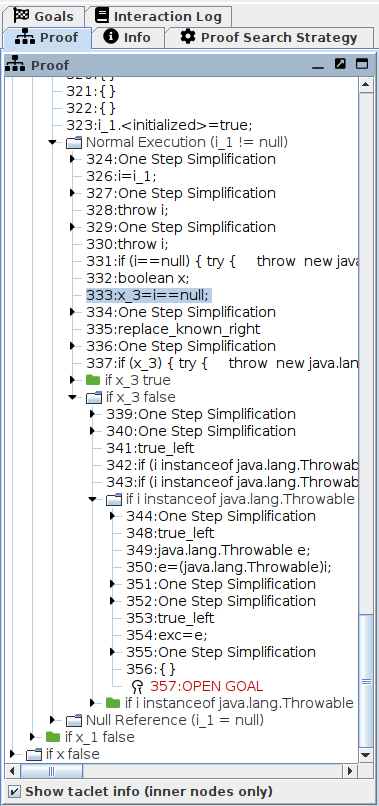
\includegraphics[width=0.357\textwidth]{../figures/proofTreeTab}
  }
    \subfigure[The \textsf{Info} tab\label{fig:prover:tab:rules}] {
    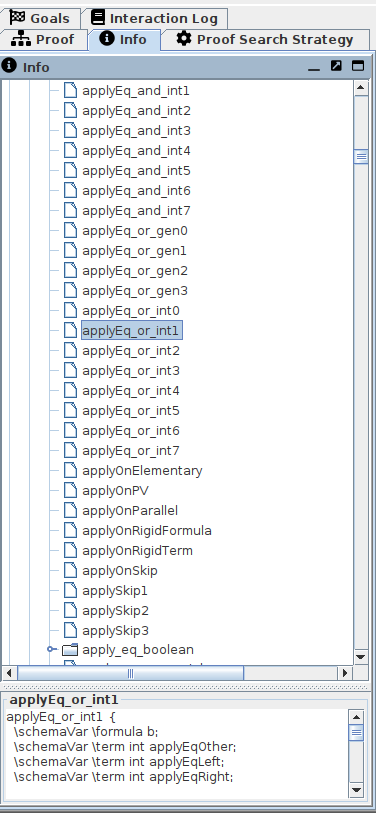
\includegraphics[width=0.35\textwidth]{../figures/infoTab}
  }  
  \subfigure[The \textsf{Proof Search Strategy} tab\label{fig:prover:tab:strategy}] {
    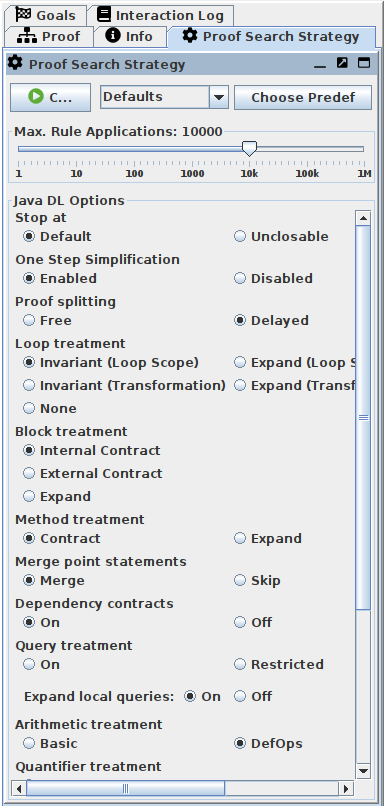
\includegraphics[width=0.35\textwidth]{../figures/strategyTab}
  }

  \caption{Selected components of the \kt\ graphical user interface}
  \label{fig:prover:components}
\end{figure}

\subsection{Configure the \kp}
\label{sec:configure}

In this section, we explain how to configure the \kp\ to follow the
tutorial and give a few explanations about the implications of the
chosen options. Most of the options are accessible via the \kp\
menu. An exhaustive list is available as part of
Appendix~\ref{app:menuOptions}. In order to verify or change some of
the necessary options, it is necessary to have a proof obligation
loaded into the \kp\ as described in Sect.~\ref{sec:loading}.

The menu bar consists of different pull-down menus:

\begin{description}
  \item[File] menu for file related actions like loading and saving
    of problems resp.\ proofs, or opening the \prm{} window
  \item[View] menu for changing the look of the \kp
  \item[Proof] menu for changing and viewing proof specific options
  \item[Options] menu for configuring general options affecting any proof
  \item[About] menu (as the name says)
\end{description}

\KeY\ provides a complete calculus for the Java Card 2.2.x version
including additional features like transactions. Further, it provides
some more concepts of real Java like class and object initialization.
This quicktour is meant to help with the first steps in the system.

For simplicity, we deactivate some advanced concepts and configure the \kp\ to
use the normal arithmetic integers to model Java integer types, which
avoids dealing with modulo arithmetics. \emph{Important:} Please
note that this configuration is unsound with respect to the Java
semantics.

In order to configure the \kp\ in this way, select
\meb{Options}{Show Taclet Options}. The dialog shows a list of
available options. 
Clicking on an option in the list also shows a short explanation
for the option.
The list below explains the options necessary for
this tutorial\footnote{App.~\ref{app:menuOptions} contains a list of
  all available options.}. Please ensure that for each option, the
value as given in parentheses directly after the option name is
selected. In case you have to change one or more values, you will have
to reload the tutorial example in order to activate them.

\begin{description}
      \item[JavaCard:] (\textsf{off}) There are two values for this option:
      \textsf{on} and \textsf{off}. Switches all
      taclets axiomatising JavaCard specific features like
      transaction on or off. 
  
   \item[initialisation:] (\textsf{disableStaticInitialisation})
      Specifies whether static initialization should be considered.

    \item[intRules:] \label{sec:integersem}
      (\textsf{arithmeticSemanticsIgnoringOF}) Here you can choose
      between different semantics for Java integer arithmetic (for
      details
      see~\cite{Schlager02,SchlagerPhD2007,KeYBook2007}). Three
      choices are offered:

      \begin{description}

      
      \item[\textsf{javaSemantics}] (Java semantics): Corresponds
        exactly to the semantics defined in the Java language
        specification. In particular this means, that arithmetical
        operations may cause over-/underflow. This setting provides
        correctness but allows over-/underflows causing unwanted
        side-effects.
      \item[\textsf{arithmeticSemanticsIgnoringOF}] (Arithmetic
        semantics ignoring overflow): Treats the primitive
        finite Java types as if they had the same semantics as
        mathematical integers with infinite range. Thus this setting
        does not fulfil the correctness criteria.
      \item[\textsf{arithmeticSemanticsCheckingOF}] (Arithmetic
        semantics prohibiting overflow): Same as above but the result
        of arithmetical operations is not allowed to exceed the range
        of the Java type as defined in the language
        specification. This setting not only enforces the java
        semantics but also ascertains that no overflow occur.
      \end{description}

\end{description}

\emph{Please} activate \tn{Minimize Interaction} in the
\texttt{Options} menu in order reduce interaction with the system.

As a last preparation step, change to the \textsf{Proof Search
  Strategy} tab in the lower left pane and choose the following setting:
\begin{itemize}

\item \textsf{Max. Rule Applications} should be set to a value greater
  or equal 500. A too low value will cause the prover to leave
  automatic mode too early. In that case, you might have to press the
  run strategy button more often than described in the tutorial.
\item \textsf{Java DL} must be selected with the following sub
  options:
  \begin{itemize}

    \item Stop at: \textsf{Default}
   \item Proof splitting: \textsf{Delayed} (\textsf{Normal} should
      also work)
    \item Loop treatment: \textsf{Invariant (Loop Scope)} 
    \item Method treatment: \textsf{Expand}
    \item Query treatment: \textsf{Expand}
    \item Expand Local Queries: \textsf{On}
    \item Arithmetic treatment: \textsf{Basic} is sufficient for this
      tutorial (when using division, modulo or similar you will need
      at least \textsf{DefOps})
    \item Quantifier treatment: \textsf{No Splits with Progs} is a
      reasonable choice for most of the time
    \item User-specific taclets: all \textsf{Off}
  \end{itemize}
\end{itemize}
 


%%% Local Variables: 
%%% mode: latex
%%% TeX-master: "quicktour"
%%% End: 


%\include{verificationOCL}

\section{Provable properties}
\label{sec:provableProp}
% evtl. Benajmins Diss zitieren
In the following, the ideas behind the various options for verification
are described informally. A formal description of the generated proof
obligations is contained in~\cite{KeYBook2016}. For
further details on the mapping between JML specifications and the
formulas of the JavaDL logic used in \KeY, please
consult~\cite{Engel05}. 

Examples of usage within the context of the case study in this
tutorial are described in Sect.~\ref{sec:application}.

\subsection{Informal Description of Proof Obligations}
The current implementation of the \kp{} generates two kinds of proof 
obligations: functional contracts and dependency 
contracts\footnote{For a detailed description of both kinds of contracts, see~\cite{Weiss2011}.}.
Method contracts describe the behavior of a method.
Properties covered by method contracts include:
\begin{itemize}
 \item \emph{properties for method specifications:} we show that a method
  \emph{fulfills} its method contract,
\item \emph{properties for class/object specifications:} we show that a method
  \emph{preserves} invariants of the object on which the call is invoked.

\end{itemize}

For the verification of programs, \emph{dependency contracts} are used to be able to rely on the 
properties of, e.g. the object invariant, in parts of the proof where 
method calls are invoked or other instructions are performed which change the memory locations on the heap. 
If these method calls only change memory locations on the heap which 
do not affect those location on which the invariant at most depends on, 
it is still possible to use the stated properties of the invariant after such a method call.
However, if the method calls also change location on the heap on which the invariant depends on, 
it is not possible to rely on those properties anymore and it has to be proven that the invariant 
still holds. For a more detailed description, see~\cite{Weiss2011}.


\subsubsection{The Logic in Use}
\label{sec:logc}

In this section, we make a short excursion to the formalism underlying
the \kt. As we follow a deduction-based approach towards software
verification, logics are the basic formalism used. More precisely,
we use a
typed first-order dynamic logic called JavaCardDL. 

We do not intend here to give a formal introduction into the
logic used, but we explain the intended meaning of the formulas. Furthermore, we
assume that the reader has some basic knowledge of classical
first-order logic. 

In addition to classical first-order logic, dynamic logic has two
additional operators called modalities, namely the diamond
$\dldia{\cdot}{\cdot}$ and box $\dlbox{\cdot}{\cdot}$ modalities. Their
first argument is a piece of JavaCard code and the second argument
an arbitrary formula. Let $p$ be a program and $\phi$ an arbitrary
formula in JavaCardDL. Then 
\begin{itemize}
  \item $\dldia{p}{\phi}$ is a formula in JavaCardDL which holds iff
    program $p$ terminates \textbf{and} in its final state formula $\phi$
    holds.  
  \item $\dlbox{p}{\phi}$ is a formula in JavaCardDL which holds iff
    \textbf{if} program $p$ terminates \textbf{then} in its final
    state formula $\phi$ holds.
\end{itemize}

The notion of a \emph{state} is a central one. A state can be
seen as a snapshot of the memory when running a program. It
describes the values of each variable or field. A formula in
JavaCardDL is evaluated in such a state. 

Let $i,j$ denote program variables. Some formulas in JavaCardDL:

\begin{itemize}
\item The formula \[
  i \keyeq 0 \keyimplies \dldia{i = i + 1;}{i \keygt 0}
  \] is a formula in JavaCardDL. The formual states:

  \begin{quote}
    If the value of $i$ is $0$, then the program $i = i + 1;$ terminates
    \emph{and} in the final state (the state reached after executing the
    program), the program variable $i$ is greater than $0$.
  \end{quote}

  The diamond operator states implicitly that the program must
  terminate normally, i.e., no infinite loops and recursions and no uncaught
  exceptions occur.

  Replacing the diamond in the formula above by a box \[
     i \keyeq 0 \keyimplies \dlbox{i = i + 1;}{i \keygt 0}
  \]
  changes the termination aspect and does not require that the program
  terminates, i.e., this formula is already satisfied if in each state
  where the value of $i$ is $0$ and \emph{if} the program $i = i + 1;$
  terminates \emph{then} in its final state $i$ is greater than $0$.

\item A typical kind of formula you will encounter is one with an update
  in front like \[ 
      \applyUp{\parUp{\elUp{i}{a}}{\elUp{j}{b}}}{\dldia{tmp = i; i =
          j; j = tmp;}{i \keyeq b \keyand j \keyeq a}}
  \] Intuitively, an update can be seen as an assignment, the two
  vertical strokes indicate that the two assignments $a$ to $i$ and
  $b$ to $j$ are performed in parallel (simultaneously). The formula
  behind the update is then valid if in the state reached executing
  the two ``assignments'', the program terminates (diamond!) and
  in the final state the content of the variables $i$ and $j$ have
  been swapped.
\end{itemize}

\subsubsection{Sequents}
\label{sec:sequents}

Deduction with the \kp\ is based on a sequent calculus for a dynamic
logic for JavaCard (JavaDL)~\cite{KeYBook2007,Beckert01}.

A sequent
has the form $\phi_1, \ldots,\phi_m\;\vdash\;\psi_1,\ldots,\psi_n\;
(m,n \geq 0)$, where the $\phi_i$ and $\psi_j$ are JavaDL-formulas.
The formulas on the left-hand side of the sequent symbol $\;\vdash\;$
are called the {\it antecedent} and the formulas on the right-hand side
are called the {\it succedent}. The semantics of such a sequent is the same as
that of the formula $(\phi_1\land\ldots\land \phi_m) \to (\psi_1
\lor\ldots\lor \psi_n)$.

% 
\subsection{Proof-Obligations}

In general, a proof obligation is a formula that has to be proved
valid. When we refer to a proof obligation, we usually mean the
designated formula occurring in the root sequent of the proof.
%
A method contract for a method $m$ of a class $C$ consists in general
of a 
\begin{description}
  \item[precondition $pre$] describing the method-specific\footnote{Additional conditions stem from invariants.}
    conditions which a caller of the method has to fulfill before calling the
    method in order to be guaranteed that the
  \item[postcondition $post$] holds after executing the method and
    that the 
  \item[assignable/modifies clause $mod$] is respected. This means
    that at most the locations described by $mod$ are modified in the
    final state. In addition, we have a
  \item[termination marker] indicating if termination of the method is
    required. Termination required (total correctness) has the termination
    marker \jn{diamond}, i.e.\ the method must terminate when the
    called in a state where the precondition is fulfilled. The marker
    \jn{box} does not require termination (partial correctness), i.e.,
    the contract must only be fulfilled if the method terminates.
\end{description}

In addition, each object $O$ has a possibly empty set of invariants
$inv_{O}$ assigned to them.

For the general description, we refer to this general kind of
contract. Mapping of JML specifications to this general contract notion
is slightly indicated in Sect.~\ref{sec:application}. More details can
be found in~\cite{KeYBook2016}.

\subsection{Application to the Tutorial Example}
\label{sec:application}

Now we apply the described proof obligations to the tutorial
example. First  we demonstrate the generation of proof obligations,
then we show how these can be handled by the \kp. Please make sure
that the default settings of the \kp{} are selected (see Chapter~%
\ref{sec:prover}) and the maximum number of automatic rule applications is
5000. Be aware that the names of the proof rules and the structure of
the proof obligations may be subject to change in the future.

\subsubsection{Method Specifications}

\paragraph{Normal Behavior Specification Case.}

In the left part of the \pob, expand the directory \jn{paycard}.
Select the class \jn{PayCard} and then the method
\jn{isValid}. This method is specified by the JML
annotation
\begin{verbatim}
   public normal_behavior
     requires true;
     ensures result == (unsuccessfulOperations<=3); 
     assignable \nothing;
\end{verbatim}

This JML method specification treats the \texttt{normal\char`\_behavior}
case, i.e., a method satisfying the precondition (JML boolean
expression following the \texttt{re\-quires} keyword) \emph{must not}
terminate abruptly throwing an exception. Further each method
satisfying the precondition must
\begin{itemize}
\item terminate (missing diverges clause),
\item satisfy the postcondition -- the JML boolean expression after
  the \texttt{ensures} keyword, and
\item only change the locations expressed in the \texttt{assignable}
  clause; here: must not change any location. The assignable clause is
  actually redundant in this concrete example, as the method is
  already marked as \texttt{pure} which implies
  \verb+assignable \nothing+.
\end{itemize}

Within \KeY, you can now prove that the implementation satisfies the
different aspects of the specification, i.e., that if the precondition
is satisfied then the method actually terminates normally and
satisfies the postconditon and that the assignable clause is
respected. In addition it is also proven that the object invariants of 
the object on which the method call is invoked are preserved.

The contracts pane in the \prm{} window offers only one proof obligation:
\jn{JML normal\_behavior opertaion contract}. 
It summarizes all parts of the specification which will be considered in the proof.

The selected contract says that a call to this method, if the object 
invariant holds  (\mea{pre} \jn{self.\textless{}inv\textgreater}), always
terminates normally and that the \jn{return} value is true iff
the parameter \jn{un\-success\-ful\-Ope\-ra\-tions} is $\leq 3$, 
Additionally, the object invariant holds after the method call, 
therefore it is preserved.
The sequent displayed in the large prover window after loading the proof
obligation exactly reflects this property.
We confirm the selection by pressing the \tn{Start proof} button.
  
Start the
proof by pushing the \tn{Start}-button (the one with the green
``play'' symbol). The proof is closed automatically by the
strategies. It might be necessary that you have to push the button
more than once if there are more rule applications needed than you
have specified with the ``Max. Rule Applications'' slider.

\paragraph{Exceptional Behavior Specification Case.}
An example of an \texttt{exceptional\_behavior} specification case can be found
in the JML specification of \jn{PayCard::charge(int amount)}. The exceptional case reads
\begin{verbatim}
  public exceptional_behavior
      requires amount <= 0;
\end{verbatim}

This JML specification is for the exceptional case. In contrast to the
\texttt{normal\_behavior} case, the precondition here states under which
circumstances the method is expected to terminate abruptly by throwing
an exception. 

Use the \prm\ (either by clicking onto the button 

\includegraphics[height=2ex]{../figures/proofManagementButton} 
or \meb{File}{Proof Management}).
Continue as before, but this time, select the method
\jn{PayCard::charge(int amount)}. In contrast to
the previous example, the contracts pane offers you three contracts: two for the
normal behavior case and one for the exceptional case. As we want to
prove the contract for the exceptional case select the contract named:
\emph{JML exceptional\_behavior operation contract}. 

The \KeY\ proof obligation for this specification requires that if the
parameter \jn{amount} is negative or equal to $0$, then the method
throw a \jn{Illegal\-Argument\-Exception}.

Start the proof again by pushing the \tn{run
  strategy}-button. The proof is closed automatically by the
strategies.

\paragraph{Generic Behavior Specification Case.}

The method specification for method \jn{PayCard::createJuniorCard()} is:
\begin{verbatim}
   ensures \result.limit==100;
\end{verbatim}
This is a lightweight specification, for which \KeY\ provides a proof
obligation that requires the method to terminate (maybe abruptly) and
to ensure that, if it terminates normally, the \jn{limit} attribute of
the result equals $100$ in the post-state. 
By selecting the
method and choosing the \emph{JML operation
  contract} in the \ctCfg, an appropriate JavaDL
formula is loaded in the prover. The proof can be closed automatically
by the automatic strategy.

\subsubsection{Type Specifications}

The instance invariant of type \jn{PayCard} is
\begin{verbatim}
    public invariant log.\inv 
    && balance >= 0 && limit > 0 
    && unsuccessfulOperations >= 0 && log != null;
\end{verbatim}

The invariant specifies that the \jn{balance} of a paycard must be non-negative, that it must be possible to charge it with some money (\jn{limit > 0}) and that the number of \jn{unsuccessfulOperations} cannot be negative. Furthermore, the invariant states that the log file, which keeps track of the transactions, must always exist (\jn{log != null}) and that the instance referred to by \jn{log} has to satisfy the instance invariant of its own class type (\verb+log.\inv+).  

The method \jn{PayCard::charge()} must preserve this
invariant unless it does not terminate. 
This proof obligation is covered by proving that 
\verb+self.<inv>+ must 
be satisfied in the precondition and must hold in the postcondition.
This has to be covered by all specification cases and is included in 
the specification in the \ctCfg (\verb+self.<inv>+ 
in the pre- and in the postcondition).

There is one exception: if a method is annotated with the keyword \jn{helper},
the proof obligation will not include the invariants. An example for such a method is \jn{LogRecord::setRecord()}.
If a method is declared as helper method, the invariant of the object on which the method is called
does not have to hold for its pre- and postcondition. For more details, see~\cite{Weiss2011}.
The advantage is a simpler proof obligation; however, the disadvantage is that
in order to show that the method fulfills its contract, it is not possible
to rely on the invariants.

In addition, invariants can also be annotated with an \texttt{accessible} clause.
In this clause, all fields and locations on which the invariant depends have to be included.
For example, the invariant of class \jn{LogRecord} is 
\begin{verbatim}
 !empty ==> (balance >= 0 && transactionId >= 0);
\end{verbatim} and it is annotated with the accessible clause
\begin{verbatim}
 accessible \inv: this.empty, this.balance, 
 transactionCounter, this.transactionId;
 \end{verbatim}

This means the invariant of \jn{LogRecord} depends at most on the fields or 
locations given in the \jn{accessible} clause. If
one of these fields is changed by a method, it has to be proven that the invariant still holds.
The accessible clause can simplify proofs because in cases where the heap is changed 
but not the mentioned fields and the validity of the invariant is proven before, 
we know that the invariant still holds.


\subsubsection{Proof-Supporting JML Annotations}

In \KeY, JML annotations are not only used to generate proof obligations but
also support proof search. An example are loop invariants. In our scenario,
there is a class \jn{LogFile}, which keeps track of a number of recent
transactions by storing the balances at the end of the transactions. Consider
the constructor \jn{LogFile()} of that class.
To prove the \jn{normal\_behavior} specification proof obligation of the method, one needs to
reason about the incorporated \jn{while} loop. Basically, there are two
ways do this in \KeY: use induction or use loop invariants. In
general, both methods require interaction with the user during proof
construction. For loop invariants, however, \emph{no interaction} is needed if
the JML \jn{loop\_invariant} annotation is used.
In the example, the JML loop invariant indicates that the 
array \jn{logArray} contains newly created entries (\jn{fresh(logArray[x])}) and that 
these entries are not \jn{null} in the array from the beginning up
to position \jn{i}:
\begin{lstlisting}
 	/*@ loop_invariant
	  @ 0 <= i && i <= logArray.length &&
	  @ (\forall int x; 0 <= x && x < i; logArray[x] != null && \fresh(logArray[x]))
	  @ && LogRecord.transactionCounter >= 0;
	  @ assignable logArray[*], LogRecord.transactionCounter;
	  @ decreases logArray.length - i; 
	  @*/	   
	while(i<logArray.length){ 
	    logArray[i++] = new LogRecord();
	}
\end{lstlisting}

If the annotation had been skipped, we would have been asked during the proof
to enter an invariant or an induction hypothesis. With the annotation no
further interaction is required to resolve the loop.


Select the contract \emph{JML normal
  behavior operation contract} \jn{LogFile}\hspace{0pt}\jn{::}\hspace{0pt}\jn{LogFile()}.

Choose \emph{Loop treatment} \emph{None} and start the prover.  
When no further rules can be applied automatically,
select the while loop including the leading updates, press the mouse
button, select the rule \emph{loopInvariant} and then \emph{Apply Rule}. This rule makes use
of the invariants and assignables specified in the source
code. 
Restart the strategies and run them until all goals are closed.

As can be seen, \KeY\ makes use of an extension to JML, which is that
\emph{assignable} clauses can be attached to loop bodies, in order to
indicate the locations that can at most be changed by the body. Doing
this makes formalizing the loop invariant considerably simpler as the
specifier needs not to add information to the invariant specifying all
those program variables and fields that are not changed by the loop.
Of course one has to check that the given assignable clause is
correct, this is done by the invariant rule. We refer
to~\cite{KeYBook2016} for further discussion and pointers on this
topic.

% \subsubsection{Using the \KeY-plugin for Eclipse}
% 
% \emph{\Large This section is currently out-of-date as the eclipse
%   plug-ins are undergoing restructuring. The principal approach is
%   still valid.}
% 
% This section will give a quick overview on the visualization
% features added by the \KeY-plugin for Eclipse. We will
% assume that the plugin has already been installed as described
% above. Start Eclipse and open the \emph{PayCard} project using
% the \emph{Import} dialog from the \emph{File} menu. The 
% \emph{paycard} directory should appear on the right hand side.
% Now open the proof visualization by selecting \emph{Other} in the
% \emph{Show View} submenu inside the \emph{View} menu. Once there
% select \emph{Proof Visualization} in the \emph{KeY} branch 
% and click \emph{OK}. Now it is time to actually open
% one of the classes, in this example we will use LogFile. 
% 
% Open the \kt\ by clicking on the \KeY-logo in the toolbar.
% As before select the \emph{PayCard} project and mark the 
% \emph{normal\_behavior speccase} for the method 
% \emph{getMaximumRecord} in the \emph{LogFile} class. Now start
% the proof. A number of open goals will remain but this time
% we won't deal with them, our focus is on the Eclipse plugin. 
% 
% It is time to take a closer look at the visualization
% options in Eclipse. Return to it and press the \emph{Show
% Execution Traces} button from the \emph{Proof Visualization}
% view. A new window should pop up with a number of execution
% traces available. Checking the \emph{Filter uninteresting traces}
% option hides those traces that appear to be irrelevant to the
% understanding of the current proof. In this case it should leave
% you with a single trace. Mark it and click \emph{OK}. Now you will
% actually see the execution trace of the selected node in the
% \emph{Proof Visualization} view. Additionally all executed statements,
% except for the last one, are highlighted in yellow inside the Java
% editor. In case of an exception the last statement is highlighted in
% dark red, otherwise in dark yellow. You can navigate through the trace
% using the buttons \emph{Step Into} and \emph{Step over}. The first one
% allows you to mark the next executed statement while the last one jumps
% over substatements and method calls. By right-clicking on a branch you
% can also choose to go into it. To return to the main execution trace
% press the \emph{Home} button. Pushing the \emph{Mark All Statements}
% button remarks all statements of the trace in the Java editor. If you
% want to clear all markers you can press the red cross. It is possible
% to receive more information on single statement, like the node at which
% the statement was executed, by moving the mouse over the marker bar
% left of the Java editor.
% 
% In case Eclipse is not available you can use a more rudimentary visualization
% built directly in the \kt. You can access it by right-clicking on a node
% and selecting \emph{Visualize}. This opens a new window with a list of traces.
% Again you have the chance to \emph{Filter uninteresting traces} and you get
% to see the trace in a tree-like structure. Statements that produced exceptions
% are highlighted in red.
% 
% The visualization options presented above concentrate on the symbolic
% execution. They allow an intuitive way for analyzing the current proof
% branch in a way that is similar to classic debuggers.


%%% Local Variables: 
%%% mode: latex
%%% TeX-master: "quicktour"
%%% End: 

% LocalWords:  postcondition



\section{Notes}

The \kt\ is continually developed, meaning that parts of this
tutorial may be outdated when you read it. Moreover, the JML semantics
are subject to discussion, and there is no formal semantics
specification for JML. Differences between the JML semantics of other
tools and the (implicitly given) semantics in \KeY\ are therefore
possible. The JML dialect of \KeY\ even extends JML in some points (as
we have seen above for \textit{assignable} clauses in
\textit{loop\_invariants}).

\KeY\ 2.10 has been tested on Linux, MacOS, and Windows.

%%% Local Variables: 
%%% mode: latex
%%% TeX-master: "quicktour"
%%% End: 


\newpage

\appendix

\section{List of Menu Options}
\label{app:menuOptions}

In the following, we describe some menu items available in the main menu
of the \kp.

\begin{description}

\item[\mea{File}] File related actions
  \begin{description}
  \item[\meb{}{Load Example}:] Opens a file browser with included example files.
  \item[\meb{}{Load}:] Loads a problem or proof file; selecting a
    directory opens the proof management window with the generated
    proof obligation for the chosen specification language
  \item[\meb{}{Reload}:] Reloads last file loaded.
  \item[\meb{}{Edit last opened file}:] If a default external editor is set, 
  this action opens the last opened file in the default external editor.  

  \item[\meb{}{Save}:] Saves the current selected proof. Note, that if
    there are several proofs loaded (see the upper left pane) only the one
    currently worked on is saved. 
   \item[\meb{}{Save as Proof Bundle}:] Saves the current selected proof as a bundle containing not only the proof itself but all source file required to reload it.
   \item[\meb{}{Quicksave}:] Saves the current selected proof to a temporary file.
   \item[\meb{}{Quickload}:] Loads the last quicksaved proof.
    
  \item[\meb{}{Proof Management}:] Allows browsing through the
    available proof obligations.
  \item[\meb{}{Load User-defined Taclets}:] Allows to activate and deactivate
    theories given as taclet collection in a \texttt{.key} file.
  \item[\meb{}{Prove}:]
  \begin{description}
    \item[\meb{}{User-Defined Taclets}:] Loads user-defined taclets 
    and generates the corresponding proof obligation.
      
    \item[\meb{}{\KeY{}'s Taclets}:] Creates proof obligations for some selected taclets.

    \item[\meb{}{Taclets using the batch mode}:]
    \end{description}
    
%   
%   \item[\meb{}{Reload Last Problem}:] 
% 		Reloads the problem you are currently working on.

  \item[\meb{}{Recent Files}:] List the last few loaded files (if
    they are still present).
    
  \item[\meb{}{Exit}:] Quits the \kp\ (be warned: the current
    proof is lost!).
  \end{description}

\item[\mea{View}] Settings influencing the look of the user interface
  \begin{description}
  \item[\meb{}{Use Pretty Syntax}:] If set, infix notation for functions and predicates are used.
  \item[\meb{}{Use Unicode Symbols}:] If set, unicode symbols instead of ASCII symbols are used for logical symbols.
  \item[\meb{}{Use Syntax Highlighting}:] Use syntax highlighting in the sequent.
  \item[\meb{}{Term labels}:] Toggle the visibility of different kinds of term labels. As explained in Sec.~\ref{sec:prover}, these do not change the semantics of the sequent but
  carry additional information that helps guide the automatic proof search and/or user.
  
  \item[\meb{}{Hide Package Prefixes}:] Print unqualified class names in the sequent instead of qualified ones.
  
  \item[\meb{}{Show Tooltips in Sequent View}:] Show a tooltip with additional information about the currently selected term.
  \item[\meb{}{Show Tooltips in Source View}:] Show a tooltip with additional information about the currently selected term.

  \item[\meb{}{Font size}] Changes the font size of the sequent and source views.

  \item[\meb{}{ToolTip options}:] Configures the tooltip shown when
    hovering over a taclet in the list of applicable taclets.
  \item[\meb{}{Visual Node Diff}:] Opens a new window which allows 
  to view the  difference between two chosen proof nodes.
  
  \item[\meb{}{Select goal}:] Select another goal in the current proof.
  \item[\meb{}{Heatmap}:] Configure heatmaps. This feature---turned off by default---highlights the most recent changes in the sequent.
  \item[\meb{}{Layout}:] Save and load the current UI layout.
  \item[\meb{}{Exploration}:] Options pertaining to proof exploration.
  \begin{description}
  	\item[\meb{}{Exploration mode}:] Enables proof exploration. This allows you to rewrite, add, or remove formulas on the sequent.
  	\item[\meb{}{Hide justification}:] Editing the sequent creates a {\em justification branch}, in which you must show that your edit does not compromise the correctness of the proof. This option allows you to hide these justification branches.
  \end{description}
  

  \end{description}

\item[\mea{Proof}] Proof specific options
  \begin{description}
  \item[\meb{}{Start}:] Run the proof (semi-)automatically w.r.t.\ 
	to current strategy options.

  \item[\meb{}{Undo Last Rule Application}:] Undo one proof step.
  \item[\meb{}{Prune proof}:] Undo all proof steps below the currently selected node.

  \item[\meb{}{Abandon Proof}:] Quits the currently active
    proof. All other loaded problems will stay in the \kp.
  \item[\meb{}{Search in proof tree}:] Opens a textfield in the proof pane, which allows to 
  search for a string in the proof tree.
  \item[\meb{}{Search in sequent view}:] Opens a window with a textfield in the lower-left 
  corner of the current goal pane, which allows to search for a string in the sequent view.
  
  \item[\meb{}{Show used contracts}:]

  \item[\meb{}{Show Active Taclet Options}:] Shows the taclet options
    chosen for the current proof.

  \item[\meb{}{Show All Active Settings}:] Opens a window displaying all settings used in the current proof.

  \item[\meb{}{Show Proof Statistics}:] Shows some general statistics
    about the proof size and interactive steps.

  \item[\meb{}{Show Known Types}:] Lists all types present in the
    current proof environment. 
    
  \item[\meb{}{Search for Counterexample}:] Searches for a counterexample to the current proof. This requires an SMT solver to be installed.
  
  \item[\meb{}{Generate Testcases}:] Generate test cases for open goals in the proof. This requires an SMT solver to be installed.

  \end{description}
  
\item[\mea{Options}] General options


  \begin{description}
  	
  \item[\meb{}{Show Settings}:] Open a settings dialog to configure \KeY's appearance.
  \item[\meb{}{Show Taclet Options}:] In the following, each taclet
    option is described briefly. The respective default settings are
    given in parenthesis. The meaning of all settings is beyond the
    scope of this quicktour. Please use the default settings unless
    you know what you are doing.
    Note that this list is not complete.

    \begin{description}
 \item[JavaCard:] (\textsf{off}) There are two values for this option:
 \textsf{on} and \textsf{off}. Switches all
 taclets axiomatising JavaCard specific features like
 transaction on or off. 

    \item[assertions:] (\textsf{on}) There exists are
      different values for this option
      \begin{description}
        \item[\textsf{on}] evaluates assert statements and raises an
          \jn{As\-ser\-tion\-Exception} if the condition evaluates to
          false. This behaviour models the behaviour of the Java
          virtual machine with assertions enabled globally.
        \item[\textsf{off}] skips evaluation of assert statement. In
          particular, the arguments of the assert statements are not
          evaluated at all. This behaviour models the behaviour of the
          Java virtual machine with assertions disabled globally.
        \item[\textsf{safe}] using this option ensures that the shown property
          is valid no matter if assertions are globally enabled or
          disabled. Proofs with this option are typically harder. 
      \end{description}
      Please note: There is no support other than option \textsf{safe}
      for enabling or disabling assertions package or class wise.

     \item[initialisation:] (\textsf{disableStaticInitialisation})
    Specifies whether static initialization should be considered.

    \item[intRules:] 
      (\textsf{arithmeticSemanticIgnoringOF}) Here you can choose
      between different semantics for Java integer arithmetic (for
      details
      see~\cite{Schlager02,SchlagerPhD2007,KeYBook2007}). Three
      choices are offered:

      \begin{description}
      \item[\textsf{javaSemantics}] (Java semantics): Corresponds
        exactly to the semantics defined in the Java language
        specification. In particular this means, that arithmetical
        operations may cause over-/underflow. This setting provides
        correctness but allows over-/underflows causing unwanted
        side-effects.
	This corresponds to the \texttt{code\char`\_java\char`\_math}
	macro in JML.
      \item[\textsf{arithmeticSemanticsIgnoringOF}] (Arithmetic
        semantics ignoring overflow, default): Treats the primitive
        finite Java types as if they had the same semantics as
        mathematical integers with infinite range. Thus this setting
        does not fulfil the correctness criteria.
	This corresponds to the \texttt{code\char`\_bigint\char`\_math}
	macro in JML.
      \item[\textsf{arithmeticSemanticsCheckingOF}] (Arithmetic
        semantics prohibiting overflow): Same as above but the result
        of arithmetical operations is not allowed to exceed the range
        of the Java type as defined in the language
        specification. This setting not only enforces the java
        semantics but also ascertains that no overflow occur.
	This corresponds to the \texttt{code\char`\_safe\char`\_math}
	macro in JML.
      \end{description}

    \item[programRules:] (\textsf{Java}) Changes between different
      program languages\footnote{Ensure that \tn{Java} is selected.}.

     \item[model fields] The semantics of model fields is given by 
     the \texttt{represents} clause in the JML specification. 
     The setting of this option decides how the represents clauses are handeled.
     It has two possible values \textsf{treatAsAxiom} 
     and \textsf{showSatisfiability}:
     \begin{description}
      \item[treatAsAxiom:] Represents clauses are seen as axioms. 
      If this option is set the satisfiability of the represents 
      clauses is not shwon and therefore it may introduce inconsistent
      specifications, e.g., he following contradictory JML clause
      will not be rejected:\\
      \texttt{//@ represents modelField == modelField + 1;}
      \item[showSatisfiability:] For every expansion of the represents 
      clause, the satisfiability of the definition has to be shown.
      Cross-definition inconsistencies can still be
      formulated, however:\\
	\texttt{//@ represents modelField1 == modelField2;}\\
	 \texttt{//@ represents modelField2 == modelField1 + 1;}
     \end{description}


     
     \item[runtime exceptions] There are two possible ways for the \kp\ in
     handling runtime exceptions -- \textsf{ban} or \textsf{allow}.
     \begin{description}
      \item[ban:] If runtime exceptions are banned, \KeY\ treats the occurence of
      runtime exceptions as irrecoverable program failure. Setting this option
      results in smaller proofs and is complete for defensive programmed programs, i.e.
      programs which do not intentionally use corner cases. 
     
      \item[allow:] If runtime exceptions are allowed, \KeY\ treats 
      runtime exceptions as defined in the Java language specification, i.e.
      implicit runtime exceptions\footnote{With implicit exceptions, we mean 
      exceptions not explicitely programmed by the developer using 
      \texttt{throw new java.lang.exception}.}
      are raised and therefore such exceptions have to be considered in the proof.
      Setting this option results in larger proofs.
     \end{description}

    \end{description}

    The current setting of the taclet options can be viewed by choosing
    \meb{Proof}{Show Active Taclet Options}.
   \item[\meb{}{Minimize Interaction}] If this option is used and the automtaic strategy is used, 
   \KeY{} tries to minimize user interaction. That means that for example, 
   if the \kp{} is able to find instantiations by itself, the user is not asked to provide them.
   \item[\meb{}{Right Click for Macros}]
   \item[\meb{}{One Step Simplification}] In the \kp\ one step simplification 
   is a mechanism to automatically apply several simplifying and normalization rule applications to the sequent. 
   For the user these rule applications are aggregated 
   into one visible rule application \textsf{One Step Simplification} 
   in the proof tree.
   Setting this option often leads to simpler sequents and results in finding a proof faster,
   but the user lacks
   transparency of the proof, because the rule applications of the one step simplifier
   are not shown in very detail compared to all other rule applications in the \kp.
  
  \item[\meb{}{Show SMT Solver Options}:] This option allows you to choose
    one or more external decision procedures that can be invoked during
    proofs and to set options for each external solver seperately. 
    There is a native interface to 
    \textsf{Simplify}. A variety of other provers
    \textsf{CVC3},  \textsf{Yices}, and \textsf{Z3}
    are directly supported via SMTLIB~\cite{RanTin-SMTLIB}. 
    In addition, translations of taclets to the SMTLIB language
    can be written to a text file (\textsf{Taclet
      Translation}) to be loaded by any SMT prover. 
    There are further options on the set of taclets to translate.
  \end{description}
  
  \item[\mea{Interaction Logging}:] These options configure the interaction log in the left pane, which logs all user interactions on the loaded proof.
  
  \item[\mea{Origin Tracking}:] These options configure the origin tracking feature. By default, a JavaDL term's origin in the JML specification is tracked throughout the proof and highlighted in the source pane when mousing over the term.
  

\end{description}
\section{List of all Strategy Tab Settings}
\label{app:strategy}
    \begin{description}
    \item[Max. Rule Applications] You can set the number $N_{aut}$ of
      automatic rule applications using the slider. Even if the
      automatic strategy can still apply rules after $N_{aut}$
      applications, automatic proving stops. 
    \item[Stop At] Choose when strategy execution shall stop.
      Possible values are \texttt{Default}: strategy stops when no
      rules are applicable or the maximal number of steps is reached and
      \texttt{Unclosable}: strategy stops in all situations when
      \texttt{Default} stops but also already when the first goal is
      encountered on which no further rule is (automatically) applicable. 
      
    \item[One-Step Simplification] When this is \texttt{Enabled}, some sequences of simplification
    steps are combined into a single proof step, resulting in shorter, but less transparent proofs.

    \item[Proof splitting] Influences usage of rules branching a
      proof tree. Only rules working on formulas not on
      programs fall under the chosen policy, i.e., program rules
      causing
      splits are still applied even if splitting is switched off. The
      values are \texttt{free} (withour restrictions), \texttt{Delayed}
      (allows still splitting but prefers other rules) and \texttt{Off} (no
      splitting).

    \item[Loop treatment] This setting determines how while-loops are
treated. They can be left untouched (\texttt{None}), handled
using stated invariant contracts, or
repeatedly unrolled (\texttt{Expand}). If handled using invariants,
you can either choose the new \texttt{Loop Scope} rule (recommended),
or the legacy \texttt{Transformation}-based rule.
    
     \item[Block treatment] It is possible to specify Java blocks with contracts. 
This option allows to set how \KeY\ treats such contracts.
\begin{description}
	\item[internal contract:] If this option is set, Java blocks are replaced by their contract.
	Three properties have to be shown in the proof:
	\begin{itemize}
		\item the validity of the contract
		\item the precondition if the contract is satisfied
		\item the use case of the contract
	\end{itemize}
	
	\item[external contract:] If this option is set, Java blocks are replaced by their contract.
	Only the precondition and the use case are shown in the current proof; the validity is outsourced to its own proof obligation which can be selected in the \texttt{Proof Obligation Browser}.
	
	\item[expand:] If this option is set, Java blocks are expanded and block contracts are not used.
\end{description}

    \item[Method treatment] Methods can also be left untouched
(\texttt{None}), have their method contracts applied
(\texttt{Contracts}), or be inlined, i.e. have the method body
expanded in place (\texttt{Expand}).

  \item[Merge-point statements] Merge-point statements are annotations in the source code. When two proof branches reach the same merge-point statement, they can be merged if this setting is set to \texttt{Merge}. If it is set to \texttt{Skip}, the merge-point statements are ignored; if it is set to \texttt{None}, the automatic proof search stops when encountering a merge-point statement. For more details on merge-point statements, see \cite{Steinhoefel2019}.
      
    \item[Dependency contracts] For the simplification of heap terms setting this option to \texttt{On}
				the information in JML's \texttt{accessible} clause is used. 
% 				For instance, consider the term<br>" +
%         		             "<center><i>f(store(heap,o,a,1))</i></center>" +
%         		             "If <i>f</i> does not depend on the location <i>(o,a)</i>, which is<br>" +
%         		             "expressed by an <tt>accessible</tt> clause, then the term can be <br>" +
%         		             "simplified to <i>f(heap)
    
    
    \item[Query treatment] A query is a method that is used as a 
    function in the logic and stems from the specification.
    There are three options for query treatment in \KeY{}:
    \begin{description}
     \item[On:] Rewrite a query to a method call such that contracts 
     or inlining (dependent on the method treatment setting) can be used.
     \item[Restricted:] Same as \textsf{On} but with restrictions:
     \begin{itemize}
      \item Priority of expanding queries that occur earlier on a branch is higher than
	    for queries introduced more recently. This approximates in a breath-first search
	    with respect to query expansion.
      \item Reexpansion of identical query terms is suppressed.
      \item A query is not expanded if one of its arguments contains a literal greater
            than a computed limit\footnote{The computation of this limit is done with 
            sophisticated methods for loop detection and would go beyond the scope of this quicktour}, 
            or smaller than a computed limit. 
            This helps detecting loops in a proof
      \item Queries are expanded after the loop body in the \texttt{Preserves Invariant}
	    branch of the loop invariant rule
      \item Queries are expanded in the \texttt{Base Case} and the conclusio of the \texttt{Step Case}
	  branch when using Auto Induction
     \end{itemize}

     \item[Off:] The query statements are ignored and the proof has to be done without using them.
    \end{description}
    In addition the \kp\ offers a setting for the expansion 
    of local queries in certain safe cases. Safe cases are:
    \begin{itemize}
     \item the return type of the expanded method is known
     \item the object on which the methodcall is invoked is self or a parent of self.
    \end{itemize}
    This setting is indepedent of the query treatment setting.


%       Queries used as terms in formulas are
%       evaluated either by symbolical execution (\texttt{Expand}), or are
%       moved to the succedent (\texttt{Prog2Succ}) so that contracts can
%       be used, or are not evaluated at all (\texttt{None}).
%       Setting \texttt{Expand Local Queries} to on results in an evaluation 
%       of the queries used as terms in formulas by symbolical execution. 
%    
   \item[Arithmetic treatment] The \kp\ has several options for the treatment of arithmetic expressions:
   \begin{description}
   \item[Basic:] Using this option, polynomial expressions are simplified. 
		 In the antecedent Gr\"{o}bner Bases are computed polynomials.
		 Linear inequations are handled using (partial) Omega procedures.

   \item[DefOps:] Using the option \textsf{DefOps}, symbols such as:\\
                \texttt{/}, \texttt{\%}, \texttt{jdiv}, \texttt{jmod}, ...\\
                \texttt{int\_RANGE}, \texttt{short\_MIN}, ...\\
                \texttt{inInt}, \texttt{inByte}, ...\\
                \texttt{addJint}, \texttt{mulJshort}, ...\\
		 are expanded.
                
    \item[Model Search:] Setting the \textsf{model search} option, 
		  the \kp\ supports non-linear equations and model search.
		  Additionally multiplication of inequations with each other
		  and systematic case distinctions  (cuts) can be performed.
                This method is guaranteed to find counterexamples for
                invalid goals that only contain polynomial (in)equations.
                Such counterexamples turn up as trivially unprovable goals.
                It is also able to prove many more valid goals involving
                (in)equations, but will in general not terminate on such goals.
                
   \end{description}

   
   \item[Quantifier treatment] Sometimes quantifiers within the
      sequent have to be instantiated. This can be either done
      manually (\texttt{None}) or automatically with different
      alternatives:
      \begin{description}
        \item[\texttt{No Splits}] Instantiate a quantifier only if
          this will not cause the proof to split.
        \item[\texttt{Unrestricted}] Instantiates a quantifier even
          when causing splits. However the startegy tries to predict
          the number of caused open branches and will prefer those
          with no or only few splits.
        \item[\texttt{No Splits with Progs}] Chooses between the
          \texttt{No Splits} and \texttt{Unrestricted} behaviour
          depending on prgrams present in the sequent. If a program is
          still present, the \texttt{No splits} behavior is
          used. Otherwise, quantifiers are instantiated without restrictions.
      \end{description}
  
     \item[Class axiom rule] This setting determines how class axioms and invariants are dealt with.
     \begin{description}
     	\item[\texttt{Free}] Class axioms are expanded freely.
     	\item[\texttt{Delayed}] Class axioms are only expanded after symbolic execution, i.e., when there are no more modalities on the sequent.
     	\item[\texttt{Off}] Class axioms are never expanded automatically.
     \end{description}
 
     \item[Auto induction] This setting can allow the \kp\ to automatically perform inductive proofs for certain formulas.
     \begin{description}
     \item[\texttt{On}] Perform inductive proofs for formulas of a certain form.
     \item[\texttt{Restricted}] Perform inductive proofs for formulas of a certain form, but only if the name of the induction variable ends with \texttt{Ind} or \texttt{IND}.
     \item[\texttt{Off}] Don't perform inductive proofs automatically.
     \end{description}
       
    \end{description}   
%   \end{description}


\section{Handy Shortcuts and Buttons}
\label{app:shortcuts}
In the following an overview of all shortcuts currently used 
in the \kp\ is given. Additional, if buttons in the toolbar exist, 
their actions are listed here as well.

\begin{tabular}{llc}
\toprule
Action/Command & Shortcut & Button in Toolbar\\

\midrule
\multicolumn{3}{l}{\textbf{File related}}\\
Load & Ctrl+O & 
\includegraphics[width=2ex]{../figures/open}\\
Reload & Ctrl+R &
\includegraphics[width=2ex]{../figures/openMostRecent}\\
Save & Ctrl+S & 
\includegraphics[width=2ex]{../figures/saveFile}\\
Proof Management & Ctrl+M & 
\includegraphics[width=10ex]{../figures/proofManagementButton}\\
Exit &Ctrl+Q& -\\
Edit last opened file & - & 
\includegraphics[width=2ex]{../figures/editFile}\\
\midrule
\multicolumn{3}{l}{\textbf{Appearance}}\\
Use pretty syntax & Ctrl+P & -\\
Font size: smaller & Ctrl+Up & -\\
Font size: larger& Ctrl+Down & -\\
\midrule
\multicolumn{3}{l}{\textbf{Proof specific}}\\
Start automatic strategy & Ctrl+S & 
\includegraphics[width=2ex]{../figures/autoModeStart}\\
Abandon task &Ctrl+W & -\\
Undo last rule application & Ctrl+Z & 
\includegraphics[width=2ex]{../figures/goalBack}\\
Search in proof tree & Ctrl+F & -\\
Search in sequent view & F3 & -\\
Prune tree below selected node & - & 
\includegraphics[width=2ex]{../figures/pruneProof} \\
SMT Solver & - &  
\includegraphics[width=10ex]{../figures/SMTButton} \\
\midrule
\multicolumn{3}{l}{\textbf{Options}}\\
Taclet options &Ctrl+T&-\\
Toggle one Step Simplifier & Ctrl+Shift+S & 
\includegraphics[width=2ex]{../figures/oneStepSimplifier}\\
\bottomrule
\end{tabular}

\section{Setting Up Own Projects}
\label{app:configuringProjects}

If not specified otherwise via a classpath directive, \KeY\ includes a
restricted set of signatures of classes and methods from the default
standard library. The current set of classes can be found at~\url{https://git.key-project.org/key-public/key/-/tree/stable/key/key.core/src/main/resources/de/uka/ilkd/key/java/JavaRedux}.

For documentation on how to set up your own classpath, see \url{https://www.key-project.org/docs/Using\%20KeY/Classpath/}.
	

%%% Local Variables: 
%%% mode: latex
%%% TeX-master: "quicktour"
%%% End: 


\bibliography{quicktour}
\bibliographystyle{alpha}

\end{document}




